\documentclass[openany]{book}
\usepackage{tabularx}
\usepackage{graphicx}

\title{Lib2geom Manual}

\newcommand{\code}[1]{\textsf{#1}}

\begin{document}
\maketitle{}

\chapter{Overview}

\section{Introduction}

This manual focuses on the lib2geom computational geometry framework.
The main goal of this framework is the eventual replacement of
Inkscape's multiple and shoddy geometry frameworks. As with any decent
module or lib, 2geom is designed to achieve the desired functionality
while maintaining a generality encouraging usage within other
applications.  The focus on robust, accurate algorithms, as well as
utilization of newer and better representations makes the lib
very attractive for many applications.

\section{Design Considerations}
2Geom is written with a functional programming style in mind.
Generally data structures are considered immutable and rather than
assignment we use labeling.  However, C++ can become unwieldy if
this is taken to extreme and so a certain amount of pragmatism is
used in practice.  In particular, usability is not forgotten in the
mires of functional zeal.

The code relies strongly on the type system and uses some of the more
'tricky' elements of C++ to make the code more elegant and 'correct'.
Despite this, the intended use of 2Geom is a serious vector graphics
application. In such domains, performance is still used as a quality
metric, and as such we consider inefficiency to be a bug, and have
traded elegance for efficiency where it matters.

In general the data structures used in 2Geom are relatively 'flat'
and require little from the memory management.  Currently most data
structures are built on standard STL headers\cite{stl}, and new and
delete are used sparingly.  It is intended for 2Geom to be fully
compatible with Boehm garbage collector\cite{boehm} though this has
not yet been tested.

\section{Toy-Based Development}
We have managed to come up with a method of library development
which is perfect for geometry - the development of toys exemplifying
a feature while the feature is perfected.  This has somewhat subsumed
the role of tests, and provides immediate motivation/reward for work.

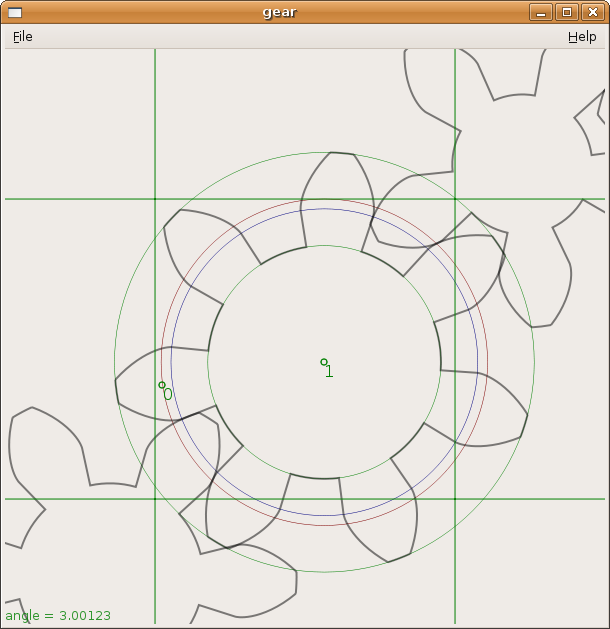
\includegraphics[width=90mm]{media/gear.png}

\chapter{Geometric Primitives}

What good is a geometry library without geometric primitives?  By this
I mean the basic stuff that every decent geometry library has -
Points/Vectors, Matrices, etc.

2geom's primitives are descendant from libNR's geometric primitives.
They have been modified quite a bit since that initial import, and
will likely change in the future.

\section{Points}

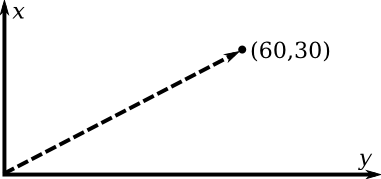
\includegraphics[height=30mm]{media/point.png}

The mathematical concepts of points and vectors are merged into the
2geom class called \code{Point}.  See Appendix A for a further
discussion of this decision.

2geom also breaks with the more traditional point \code{struct} with
\code{.x} and \code{.y} fields.  Rather, each 2geom point has a 2
element array of coordinates.

We found that the availability of \code{.x} and \code{.y} encouraged
people to attempt to inline geometry operations rather than using the
operators, perhaps in pursuit of a performance enhancement.  By using
an array, we encourage people to think about \code{Point}s as
symmetric objects and discourage direct use of the components.  We
still provide direct access for the rare occasion that it is needed.
Even in these cases, the array method prevents bugs by encouraging
iteration over the array rather than explicit element reference.

\section{Transformations}

Affine transformations are either represented with a canonical 6
element matrix, or special forms.

\subsection{Scale}

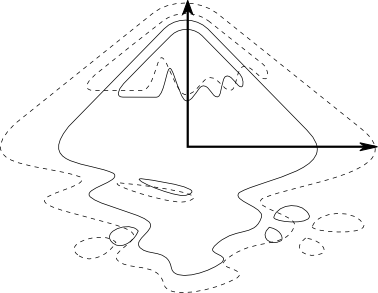
\includegraphics[height=50mm]{media/scale.png}

A \code{Scale} transformation stores x and y scaling factors.

\subsection{Rotate}

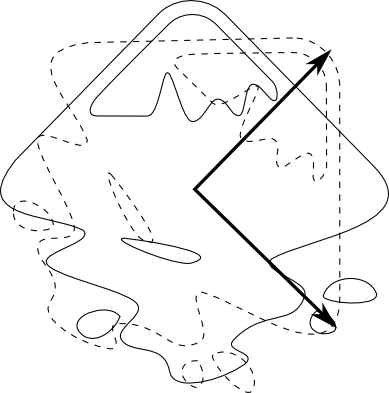
\includegraphics[height=50mm]{media/rotate.png}

A \code{Rotate} transformation uses a vector(\code{Point}) to store
a rotation about the origin.

In correspondence with mathematical convention (y increasing upwards),
0 degrees is encoded as a vector pointing along the x axis, and positive
angles indicate anticlockwise rotation.  So, for example, a vector along
the y axis would encode a 90 degree anticlockwise rotation of 90 degrees.

In the case that the computer convention of y increasing downwards,
the \verb}Rotate} transformation works essentially the same, except
that positive angles indicate clockwise rotation.

\subsection{Translate}

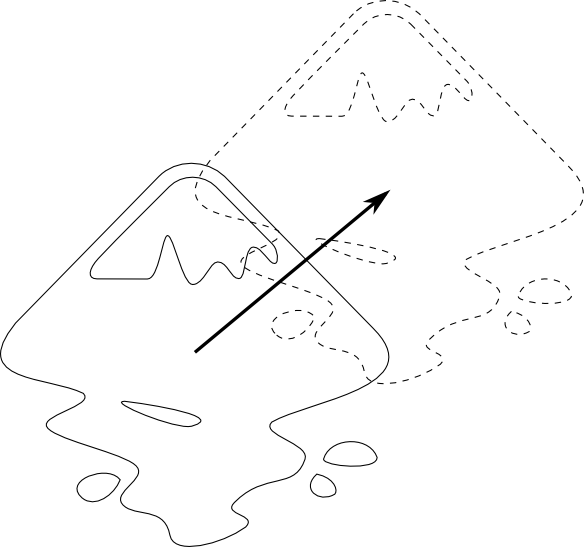
\includegraphics[height=70mm]{media/translate.png}

A \code{Translate} transformation is a simple vector(\code{Point})
which stores an offset.

\subsection{Matrix}

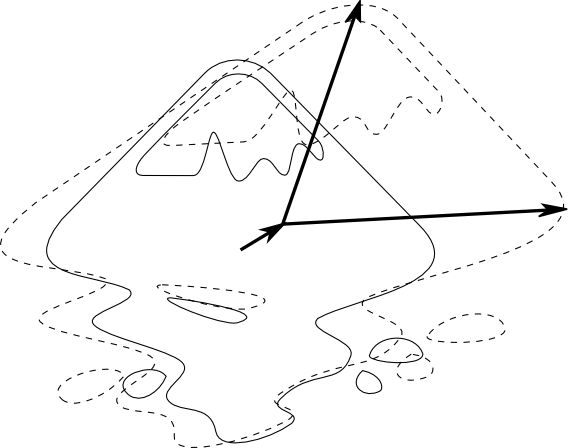
\includegraphics[height=70mm]{media/matrix.png}

A \code{Matrix} is a general affine transform.  Code is provided for
various decompositions, constructions, and manipulations.  A
\code{Matrix} is composed of 6 coordinates, essentially storing the
x axis, y axis, and offset of the transformation.  A detailed
explanation for matrices is given in Appendix B.

\section{Bounding Structures}

2geom currently provides two classes for storing approximate bounding
regions - \code{Rect} and \code{ConvexHull}.  These are mostly intended
for use in optimization, however provide manipulations suitable for
other uses.

\subsection{Rect}

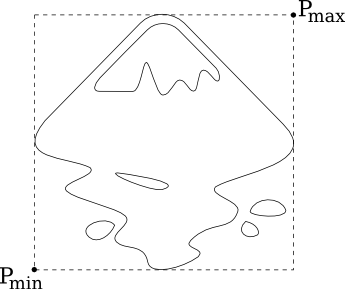
\includegraphics[height=50mm]{media/rect.png}

\code{Rect}s are rectangles with all sides parallel to the axes. They
are defined with two points, each an opposing corner.

\subsection{ConvexHull}

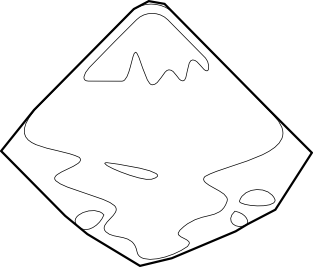
\includegraphics[height=50mm]{media/convex.png}

Currently there are two implementations:
\begin{description}
\item[convex-hull.h] is the inkscape version using rectangles.
\item[convex-cover.h] is partial implementation done with a set of points in clockwise direction.
\end{description}

\subsubsection{Operations}
\begin{description}
\item[empty:] contains no points
\item[singular:] contains exactly one point
\item[linear:] all points are on a line
\item[area:] area of the convex hull
\item[furthest:] furthest point in a direction (log time)
\item[intersect:] do two convex hulls intersect?
\item[intersection:] find the convex hull intersection
\item[merge:] find the convex hull of a set of convex hulls
\end{description}

\chapter{Paths}

Our original attempt at a \code{Path} class was to store parallel
lists of curve types and handles.  This turned out to be very clumsy,
so MenTaLguY wrote a new path-framework, called Path2.  Currently the
files are still called this, even though Path1 has been mostly
removed.

A \code{Path} is an ordered set of \code{Curve}s.  A \code{Path} in
Inkscape is drawn in a single fill and stroke.

This allows us lots of flexibility with what sort of elements we can
'understand', while only taking slightly more memory than a sequence
of points in the poly line or poly bezier case. 

\section{Curves}
2Geom has a diversity of curve types and conversions between them.

Curves define a continuous segments which yields points for values of
t in the range of [0,1].  The start-point is at t=0, and the endpoint
at t=1.

We require that each \code{Curve} implements virtual functions which
allow for traversers of a path to perform generic operations.  All
curves must provide functions which give a position and gradient of a
$t \in [0,1]$, bounds functions, and conversion to s-basis.

\subsection{Bezier Curve}
We use a \code{Bezier} curve class to store lines and quadratic/cubic
beziers.  This flexibility is attained by templating on order -
\code{Bezier$<1>$} is a line segment, \code{Bezier$<2>$} is a quadratic
bezier, and \code{Bezier$<3>$} is a cubic bezier.

Bezier curves have some nice properties:
\begin{itemize}
\item Affine transforming the handles also affine transforms the values.
\item The convex hull of the handles encompasses the curve.
\end{itemize}

\subsection{SVG Elliptical Arc}
The \code{SVGEllipticalArc} curve class is implemented for support of
the SVG elliptical arc.  See the svg documentation for details on this
curve.

\subsection{S-Basis Curve}
The \code{SBasisCurve} wraps the \code{MultidimSBasis$<2>$} class
described later.

\subsection{Possible Future Curve Types}
\begin{itemize}
\item Clothoids / Raphoids
\item NURBS
\end{itemize}

\chapter{S-Power-Basis Form}

2Geom provides a very powerful algebra for modifying paths.  Although
paths are kept in an extended SVG native form where possible, many
operations require approximation.  To do this we can convert a path
into a sequence of s-power basis polynomials, henceforth referred to
as s-basis, perform the required operations and convert back,
approximating to a requested tolerance as required.

The precise details of the s-basis form are beyond the scope of this
manual, the interested reader should consult \cite{SanchezReyes1997,SanchezReyes2000,SanchezReyes2001,SanchezReyes2003,SanchezReyes2004}.
An elementary, functional description is given in Appendix C.

Geometrically important properties:
\begin{itemize}
\item exact representation of bezier segments
\item low condition number on bezier conversion.
\item strong convergence guarantees
\item $C^0$ continuity guarantee
\end{itemize}

The following operations are directly implementable and are very efficient:
\begin{itemize}
\item fast conversion from all svg elements
\item basic arithmetic - $+$, $-$, $\times$, $\div$
\item algebraic derivative and integral
\item elementary trigonometric functions: $\sqrt{\cdot}$, $\sin(\cdot)$, $\cos(\cdot)$, $\exp(\cdot)$
\item efficient degree elevation and reduction
\item function inversion
\item exact solutions for many non trivial operations
\item root finding
\item composition
\end{itemize}

All of these operations are fast.  For example, multiplication of two
beziers by converting to s-basis form, multiplying and converting back
takes roughly the same time as performing the bezier multiplication
directly, and furthermore, subdivision and degree reduction are
straightforward in this form.

\section{Implementation}
As described in Appendix C, SBasis functions have the form $f(t) \rightarrow y$.
Just S-Basis functors (in the C++ sense) alone are not enough to perform
useful geometric operations.  There are quite a few 2geom classes to
address these needs.

\subsection{SBasis}
The \code{SBasis} class provides the most basic function form,
$f(t) \rightarrow y$.  This is useful in its own right, as well as being an
element of constructing more complicated forms.  \code{SBasis} are made
up of \code{BezOrd}s, which store from/to values for each polynomial
coefficient.

\subsection{MultidimSBasis}
The \code{MultidimSBasis$<>$} class provides a convenience wrapper
around multiple sbasis at once, to produce multiple values for a t-value.
$f(t) \rightarrow (v_0, v_1, .. v_d)$.  A special case is \code{MultidimSBasis$<2>$},
a 2 diminsional curve.

\subsection{SBasis2D}
SBasis2D provides a multivariate form - functions of the form
$f(u,v) \rightarrow z$.  These can be used for arbitrary distortion
functions (take a path $p(t) \rightarrow (u,v)$ and a pair of surfaces
$f(u,v),g(u,v)$ and compose: $q(t) = (f(p(t)), g(p(t)))$.

Subdivision for surfaces may be done with either quadtrees or kd-trees.

\subsection{Piecewise SBasis}
The piecewise sbasis class, \verb#pw_sb#, manages a sequence of SBasis
segments and the 'cuts' between them.  These cuts are time values which
separate the different SBasii.  This function representation allows for
more interesting functions, as it provides a viable output for operations
such as inversion, which may require multiple SBasis to properly invert
the original.

As for technical details, while the actual SBasis segments begin on the
first cut and end on the last, the function is defined throughout all
inputs by extending the first and last segments.  The exact switching
between segments is arbitrarily such that beginnings (t=0) have
preference over endings (t=1).  This only matters if it is discontinuous
at the location.

$$
f(t) \rightarrow \left\{ 
\begin{array}{cc}
s_1,& t <= c_2 \\
s_2,& c_2 <= t <= c_3\\
\ldots
s_n,& c_n <= t
\end{array}\right.
$$

\subsection{Multidim Piecewise SBasis}
This is like Multidim SBasis, only for the piecewise type.  Multidim
SBasis might be subsumed by this class, or they will both be replaced
by a general Multidim template.

\chapter{2D databases}

2Geom provides an implementation of a 2D database using quad trees and
using a list.  Quad trees aren't the best data-structure for queries,
but they usually out perform the linear list.  We provide a
standard interface for object databases with performance guarantees
and provide a set of useful operations Operations:

\begin{description}
\item[Insert:] given a bounding box and a 'reference', insert into the db
\item[Delete:] given a bounding box and a 'reference', delete from the db
\item[Search:] given a box, find all objects that may interact with this box
\item[Cast:] given a path (including rays) return a list of objects that interact with the path, roughly sorted by path order
\item[Shape query:] given a closed path, find all objects whose bounding boxes intersect path.  (this and cast are nearly the same)
\item[Nearest:] given a point (or maybe box) find the nearest objects, perhaps as a generator to get all objects in order.  To do this, we walk around the quad tree neighbourhood, pushing all the elements into a priority queue, while the queue is empty, move out a bit.  Nearest could be manhattan, max norm or euc?
\item[Binary:] take two dbs, generate all pairs that have intersecting boxes.
\item[Sweep:] traverse the tree in say y order, maintaining a y-range of relevant objects. (to implement sweepline algorithms)
\item[Walk:] traverse the tree in an arbitrary order.
\end{description}

\chapter{Acknowledgements and history}

2Geom is a group project, having many authors and contributors.  The
original code was sketched out by Nathan Hurst and Peter Moulder for
the Inkscape vector graphics program to provide well typed, correct
and easy to use C++ classes.  Since then many people have refined and
debugged the code.  One of the earliest C++ification projects for
inkscape was replacing NRPoint with NR::Point.

A conspicuous absence was a Path datatype, and indeed Inkscape
developed at least 3 different internal path datatypes, plus several
others in related projects.  Considering the core importance of path
operations in vector graphics, this led to much reimplementation of
algorithms, numerous bugs, and many round trips converting between
forms.

Many attempts have been made to try and develop a single path data
structure, but all were fated to sit in random SCMs scattered across
the web.

Several unrelated projects had copied out various portions of the NR
code from Inkscape and in 2006 MenTaLguY and Nathan felt that it was
time to separate out the geometry portions of inkscape into a
separate library for general use and improvement.  The namespace was
changed from NR to Geom and a prototype for paths sketched out.
Nathan studied the state of the art for computational geometry whilst
mental focussed on the design of Paths.

Before the remerging of 2Geom with the inkscape svn HEAD it was felt
that a few smaller projects should be ported to use 2Geom.  Michael
Wybrow's libavoid advanced connector routing system was ported first.

--now.

\pagebreak

\section{People who have contributed to 2Geom}
\begin{description}
\item[Aaron C. Spike]
\item[Alex Mac]
\item[Fred:] livarot
\item[Javier Sanchez-Reyes]
\item[Jean-Francois Barraud]
\item[Jonathon Wright]
\item[Joshua Blocher]
\item[Kim Marriott]
\item[MenTaLguY]
\item[Michael J. Wybrow]
\item[Michael G. Sloan]
\item[Nathan J. Hurst]
\item[Peter J. R. Moulder]
\end{description}

\chapter{Appendix}
\renewcommand{\thesection}{\Alph{section}}

\section{Geometric Points}
In standard geometry points and vectors are quite distinguished - a  
point is a location, whereas a vector is an unbased direction and
magnitude.  Allowed operations on vectors and points also vary:

\begin{tabular}{r l}
  $P - P$ & $= V$ \\

  $P - P$ & $= V$ \\

  $P + V$ & $= P$ \\

  $P - V$ & $= P$ \\

  $V + V$ & $= V$ \\

  $V - V$ & $= V$ \\

  $V \times S$ & $= V$ \\

  $V \div S$ & $= V$ \\
\end{tabular}

Here, $P$ represents points, $V$ represents vectors, and $S$ scalars.

Ideally we would render these restrictions in code, as they would
reinforce algorithm correctness.  This is because as far as arithmetic
operations go, the above are all that you sanely require, unless you
are prematurely optimizing.

\section{Understanding Matrices}

\section{S-Power-Basis Explanation}

\section{Concepts}

The C++ Standard Template Library\cite{stl} introduces the notion of
\emph{concepts}\cite{stl_concepts}, which specify families of types related
by a common interface.  In template-based programming with the STL, concepts
serve a similar purpose to type classes in Haskell.  While, unlike Haskell's
language-level support for type classes, concept-checking is not directly
supported by the C++ compiler or language, C++ libraries have been written
which use template techniques to provide compile-time checking and enforcement
of concepts\cite{boost_concept_check}.

There are several important lib2geom concepts in this sense:

\subsection{ScalarFunction}

\subsubsection{Description}

Scalar functions are C++ function objects which behave like functions
with type {\tt double (double)}.  They take a single time value and return
a scalar, and are defined over at least the interval $[0, 1]$.

\subsubsection{Refinement of}

\subsubsection{Associated types}

\subsubsection{Notation}

\begin{tabular}{r l}
  {\tt X} & A type which models ScalarFunction \\
  {\tt a} & An object of type {\tt X} \\
  {\tt t} & A time value of type {\tt double} \\
  {\tt n} & A count of type {\tt unsigned int} \\
\end{tabular}

\subsubsection{Definitions}

\subsubsection{Valid expressions}

\begin{tabularx}{300pt}{X l X l}
  Name & Expression & Type requirements & Return type \\
  Evaluate & {\tt a(t)} & & {\tt double} \\
  Evaluate & {\tt a.valueAt(t)} & & {\tt double} \\
  Evaluate with derivatives & {\tt a.valueAndDerivativesAt(t, n, out)} & {\tt out} should be a model of OutputIterator whose {\tt value\_type} is convertible to & {\tt void} \\
  Range & {\tt a.fastRange()} & & {\tt Range} \\
  Range & {\tt a.exactRange()} & & {\tt Range} \\
  SBasis & {\tt a.sbasis()} & & {\tt SBasis} \\
  Subdivide & {\tt a.subdivide(start, end)} & & {\tt Piecewise<X>} \\
\end{tabularx}

\subsubsection{Expression semantics}

\begin{tabularx}{300pt}{X l l X l}
  \bf{Name} & \bf{Expression} & \bf{Precondition} & \bf{Semantics} & \bf{Postcondition} \\
  Evaluate & {\tt a(t)} & $0\le t\le 1$ & Returns the value of the function at $t$; the function must be exact at $t = 0$ and $t = 1$ and defined over the interval $0\le t\le 1$ & \\
  Evaluate & {\tt a.valueAt(t)} & $0 \le t \le 1$ & Returns the value of the function at {\tt t}; the function must be exact at $t = 0$ and $t = 1$ and defined over the interval $0 \le t \le 1$ & \\
  Evaluate with derivatives & {\tt a.valueAndDerivativesAt(t, n, out)} & $0 \le t \le 1$ & Evaluates the function and the first n derivatives at {\tt t}, writing them to {\tt out} & $n + 1$ values have been written to {\tt out} \\
  Range & {\tt a.fastRange()} & & The result should be a {\tt Range} which includes the function's range & \\
  Range & {\tt a.exactRange()} & & The result should be a {\tt Range} representing the exact range of the function & \\
  SBasis conversion & {\tt a.sbasis()} & & The result should be an sbasis approximation of the function & \\
\end{tabularx}

\subsubsection{Complexity guarantees}

\subsubsection{Invariants}

\subsubsection{Models}

\subsection{Curve}

\subsection{UVFunction}

\section{Location Sequences}

Many algorithms are more efficient on a sorted sequence of locations,
than calling the function repeatedly for each.  So we have algorithms
that take a sequence of locations, assumed in order, and perform an
action on those.  For example, cutting a path at one location is
basically linear in the number of path segments, but cutting a path in
10 locations is still about the same amount of work.  Similarly,
working out the arc length for a location is about the same amount of
work as working out the arc length for 1000 locations on that path.

Many operations are best described as returning an ordered set of
locations - for example, we have a function which returns
intersections between two paths.  rather than return just one
intersection, we might return all intersections, either in order along
the path, or in order of distance along other path.

Think about dashes: a dash is a fixed arclength offset.  So rather
than getting the location for a point at arc length 1, at arc length
2, 3, 4.. to the length of the curve, instead we just ask for all of
these, and the algorithm can chug along the curve outputting the
answer for each.  the reason it is faster is because to work out the
location at arc length say 100, we basically need to work out the
length for many spots up to 100.

Perhaps we then want to split the curve at each of those points.  To
split a segment at a location first requires finding that segment,
then splitting it and finally constructing a new path to output a whole
new path so we can fit the two new segments in.  If we started at the
beginning, and split at the first location, that would be n+1 steps - n
segs in the original, plus an extra one.  If we wanted to split at 100
points, it would be n+1 steps for the first, n+2 for the
second... n+100 steps for the last, this would take a total of 100n +
100*101/2 steps!  Whereas, if we split as we went along, it would take
just n+100 steps.

The downside is that I'll probably not provide a separate split
routine that takes a single point, to discourage people from making
exactly that mistake.

\end{document}
